
\fancyhead[C]{Section 15.5}
\fancyhead[R]{\dayeighteen}

\section*{\centering Chapter 15.5: Triple Integrals}
\textbf{I1: Double \& Triple Integrals.} I can set up double and triple integrals as iterated integrals over any region. I can sketch regions based on a given iterated integral.

\textbf{I2: Iterated Integrals.} I can compute iterated integrals of two and three variable functions, including applying Fubini's Theorem to change the order of integration of an iterated integral.

\subsection*{Mechanics}
\begin{enumerate}
    \item Triple integrals can compute volumes, just like double integrals can, so when might you prefer to use one over the other? Give an example of a solid whose volume is easier to compute with a double integral, and vice versa. 
    
    \item Evaluate the triple iterated integral
	   \begin{equation*}
	       \int_{-1}^1\int_{0}^4\int_0^1 (z^3-4x^2y)\ dz\ dy\ dx
	   \end{equation*}
	Recall that to evaluate the innermost integral, treat both $x$ and $y$ as constants and take the antiderivative with respect to $z$.
	
	Describe the region of integration.
       	
	\item Set up a triple iterated integral for $\iiint_E z\ dV$, where $E$ is the solid tetrahedron in the first octant bounded above by $x+y+z=1$. It may be helpful to make a sketch of the solid.
    
    \item Set up integrals that would calculate the volume of the region below, using the specified orders of integration.
	\begin{center}
		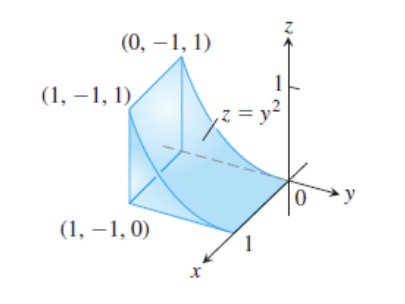
\includegraphics[scale=0.45,alt={region above the square with -1<y<0,0<x<1 under the surface z=y^2}]{15_5pic.PNG}
	\end{center}
	
	\begin{multicols}{5}
    \begin{enumerate}
		\item $dy \ dz \ dx$
		\item $dy \ dx \ dz$
		\item $dx \ dy \ dz$
		\item $dx \ dz \ dy$
		\item $dz \ dx \ dy$
	\end{enumerate}
    \end{multicols}
\end{enumerate}

\pagebreak

\subsection*{Applications}
\begin{enumerate}[resume]
    \item A solid with density $\delta(x, y, z) = 3x^2yz$ is bounded below
by the plane $z = 0$, on the sides by the elliptical cylinder
$x^2 + 4y^2 = 4$, and above by the plane $z = 2 − x$. Set up
all of the necessary triple integrals to compute its center
of mass. You do not need to compute any integrals (unless you want to). It may be helpful to sketch the solid first.

    \item The triple integral below represents the volume of a particular solid, called the \textit{Steinmetz} solid:
    \begin{equation*}
        \int_{-1}^1\int_{-\sqrt{1-x^2}}^{\sqrt{1-x^2}}\int_{-\sqrt{1-x^2}}^{\sqrt{1-x^2}}dy \ dz \ dx
    \end{equation*}
    Perform this integral, and then unravel the bounds to realize it as the intersection of two simpler solids. Though mathematician Charles Steinmetz is cited with the study of this in the 17/18th century, evidence of its study traces back to ancient Greece and China, as well as the early Renaissance. Can you spot the Steinmetz solids in the following pictures?

\begin{minipage}{.45\textwidth}
  \centering
  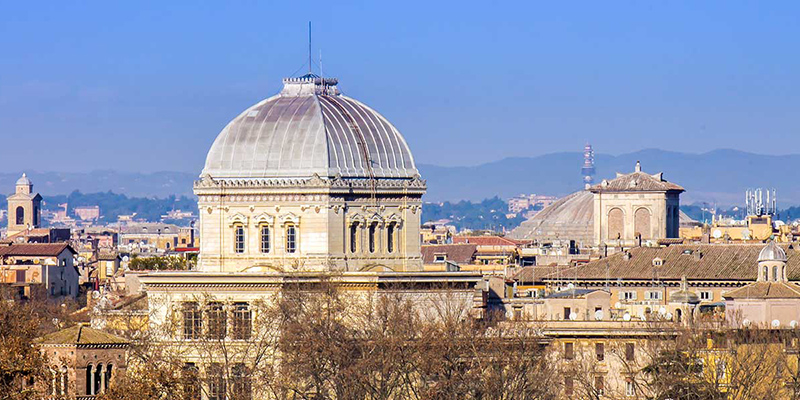
\includegraphics[width=.8\linewidth,alt={synagogue in rome with a Steinmetz shaped dome}]{Jewish-Synagogue-Rome.jpg}
\end{minipage}%
\begin{minipage}{.45\textwidth}
  \centering
  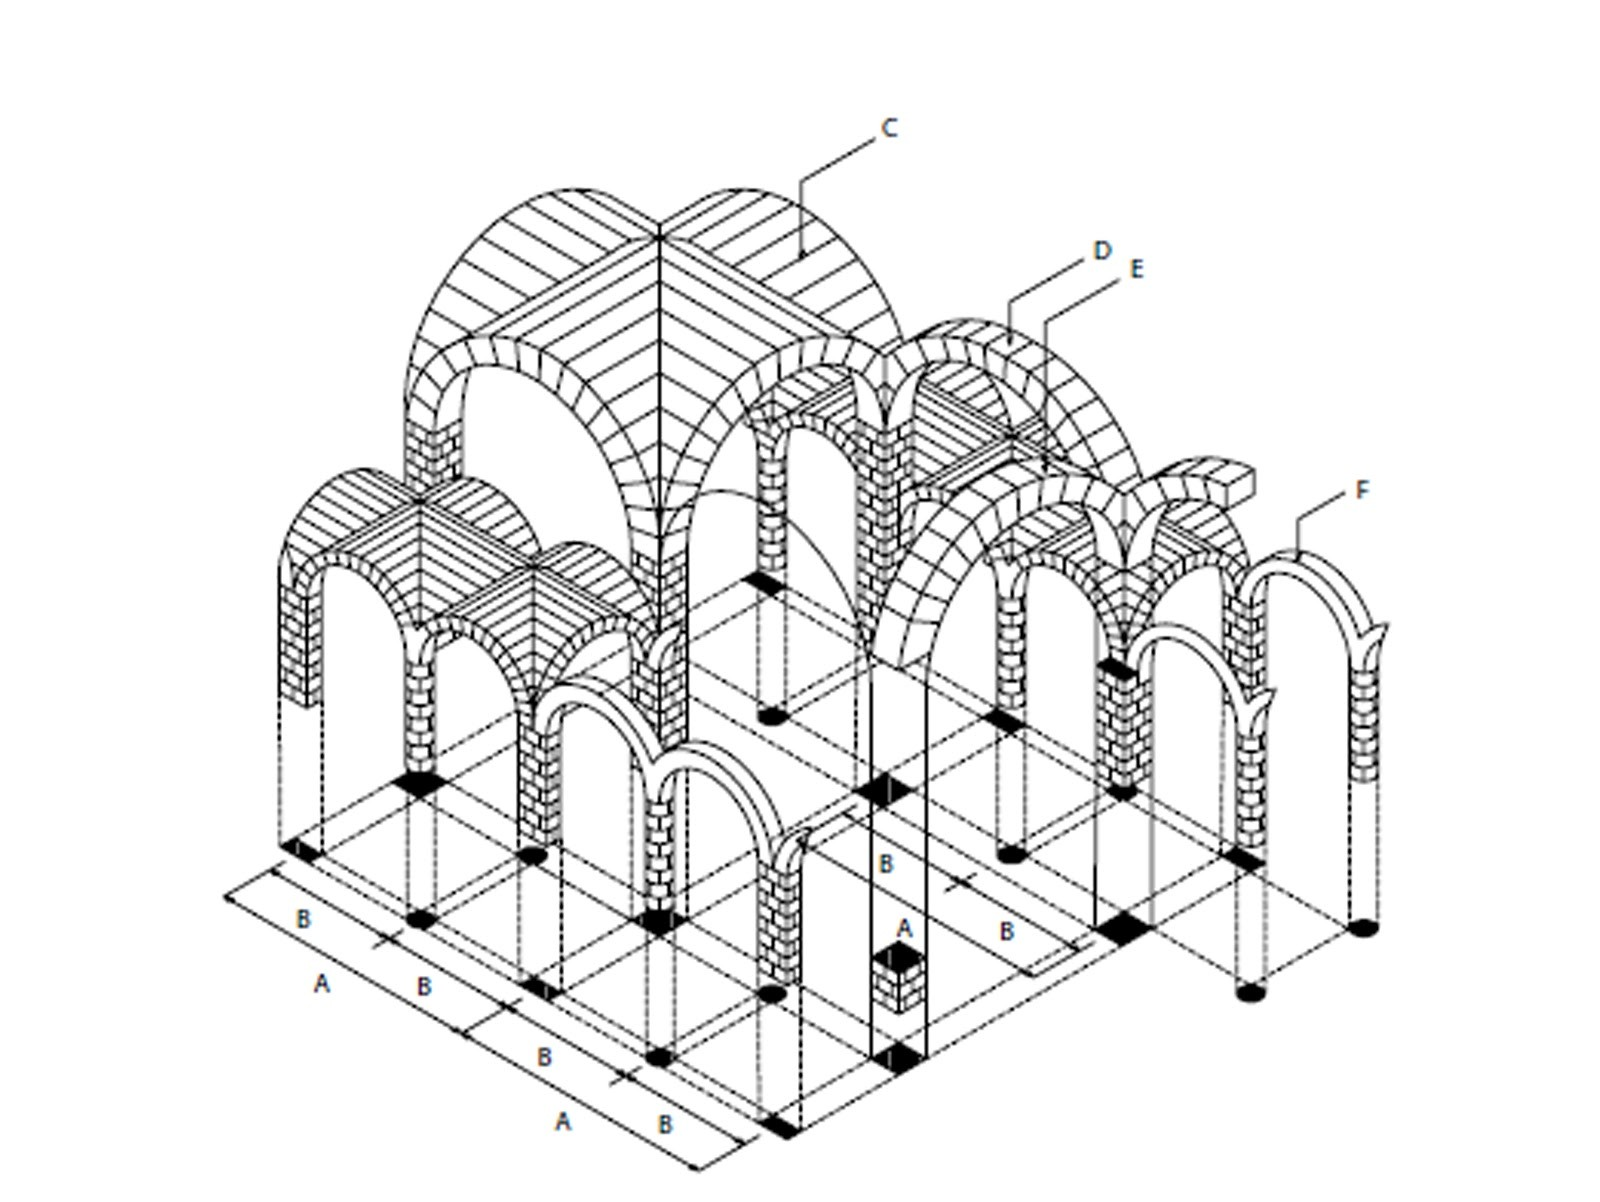
\includegraphics[width=.9\linewidth,alt={architectural diagram of a groined vault ceiling}]{groin vault.jpg}
\end{minipage}
\end{enumerate}
\subsection*{Extensions}
\begin{enumerate}[resume]
	
		
	\item Use a clever swap of the order of integration to evaluate 
    \begin{equation*}
    \int_0^9\int_{\sqrt{z}}^3\int_0^yz\cos(y^6)dxdydz
    \end{equation*}
    \textit{[Hint: Note that the both the function and bounds do not detect the variable $x$, so you can rearrange to take care of the $x$-integral first. Now note that $\cos(y^6)$ has no elementary antiderivative.]}
    
	
	\item Let $D$ be the region bounded by the paraboloid $z=x^2+y^2$ and the 
	plane $z=2y$, i.e. \[D=\{(x,y,z) \in \R^3 \mid x^2+y^2 \leq z \leq 2y\}.\] 
	Write triple iterated integrals in the orders $dz\ dy\ dx$ and  $dx\ dz\ dy$
	that give the volume of $D$.  Can you write a single triple iterated integral for this volume using any other orders of integration?

%%%%%%
\end{enumerate}

\iftoggle{answers}
{
	\begin{center}{\large \textbf{Math 2551 Worksheet Answers: Triple Integrals}}
	\end{center}

\begin{enumerate}
	\item $\dfrac{-58}{3}$, region of integration the rectangular prism $[-1,1]\times[0,4]\times[0,1]$ or $-1\leq x \leq 1, 0\leq y \leq 4, 0\leq z\leq 1$.

	\item Various possibilities depending on order of integration.  E.g \[\int_0^1 \int_0^{1-x} \int_0^{1-x-y}\ z\ dz\ dy\ dx \]

	\item 
	\begin{enumerate}
		\item $\displaystyle\int_0^1 \int_0^1 \int_{-1}^{-\sqrt z}\ dy \ dz \ dx $
		\item $\displaystyle\int_0^1 \int_0^1 \int_{-1}^{-\sqrt z}\ dy \ dx \ dz  $
		\item $\displaystyle\int_0^1 \int_{-1}^{-\sqrt z} \int_0^1\ dx \ dy  \ dz  $
		\item $\displaystyle\int_{-1}^0 \int_0^{y^2} \int_0^1 \ dx \ dz \ dy$
		\item $\displaystyle\int_{-1}^0  \int_0^1  \int_0^{y^2}\ dz \ dx \ dy$
	\end{enumerate}

	\item $\Ds \int_{-1}^1 \int_{1-\sqrt{1-x^2}}^{1+\sqrt{1-x^2}} \int_{x^2+y^2}^{2y} dz\ dy\ dx$.
	
		$\Ds \int_{0}^{2} \int_{y^2}^{2y} \int_{-\sqrt{z-y^2}}^{\sqrt{z-y^2}} dx\ dz\ dy$.
		
		Yes, all orders of integration result in a single iterated integral.
\end{enumerate}
}{}
\iftoggle{solutions}
{
Solutions go here in the same format.
}{}
